\section{Introduction}
L'objet de ce projet est de grouper au sein de différents clusters un ensemble de séries temporelles, et ce faisant d'estimer le modèle statistique décrivant les séries temporelles de chaque cluster. 
Pour conduire nos estimations, nous nous plaçons dans le cadre bayésien et utilisons des méthodes de simulation de Monte Carlo et chaîne de Markov cachées.
\newline
Soit ($y_{i,t}$), \textit{t=1,...,T}, une série temporelle multiple, parmi N autres series temporelles \textit{i=1,...,N}, on fait l'hypothèse que ces séries appartiennent à K clusters différents, et que toutes les séries temporelles appartenant à un cluster $\textit{k}$ sont décrites par le même modèle statistique avec un paramètre spécifique au groupe, $\theta_k$. L'appartenance à un groupe \textit{k} pour chaque série temporelle \textit{i} est inconnue à priori et est estimée en même temps que les paramètres $\theta_k$. On fait de plus l'hypothèse que les paramètres $\theta_k$ sont propres à chaque cluster. 
\newline
On introduit le vecteur $S = (S_1,S_2,...,S_N)$ où $\forall i \in 1,..,N$, $S_i$ $\in 1,...,K$ indique le groupe auquel appartient la série temprelle $i$, ainsi que le vecteur $\phi = (\eta_1, ..., \eta_K)$ où $\eta_k$ indique la proportion de série temporelle appartenant au cluster $k$
\newline
En utilisant un algorithme de MCMC, nous allons itérativement estimer le vecteur $S$, puis les vecteurs $\theta$ et $\phi$.

\section{Le modèle}
\subsection{Point de vue théorique}

Pour $i = 1,..,N$, la densité de $y_i$ conditionnellement à $\theta_{S_i}$ s'écrit :

\begin{equation}
\textit{$p(y_i | \theta_{S_i})$} = \prod_{t=1}^{T} \textit{$p(y_{i,t}|y_{i,t-1},..,y_{i,0},\theta_{S_i})$}
\end{equation}

Où \textit{$p(y_i|y_{i,t-1},..,y_{i,0},\theta_{S_i})$} est une densité connue qui dépendra du modèle choisi.
\newline
Par conséquent, 
\begin{equation}
\textit{$p(y_i | S_i, \theta_1,...,\theta_K) =  p(y_i | \theta_{S_i})$} = \left\{\begin{array}{ll}
  \textit{$p(y_i | \theta_{1})$}   & \mbox{si } S_i = 1  \\
  ...                                         \\
  \textit{$p(y_i | \theta_{K})$}   & \mbox{si } S_i = K
\end{array}\right.
\end{equation}
\newline
Ensuite, on détermine un modèle probabiliste pour la variable $S = (S_1,..,S_N)$. On fait l'hypothèse que les $S_1, S_2,..,S_N$ sont deux à deux à prori indépendants et pour tout $i = 1,..,N$ on définit la probabilité à priori $Pr(S_i = k)$, la probabilité que la série temporelle $i$ appartienne au cluster $k$. On fait l'hypothèse que pour toute série $i$, on n'a à priori aucune idée d'à quel cluster elle appartient. Dès lors,
\begin{equation}
Pr(S_i = k | \eta_1,..,\eta_K) = \eta_k
\end{equation}
La taille des groupes $(\eta_1,..,\eta_K)$ est à priori inconnue et est estimée grâce aux données.

\subsection{L'algorithme de MCMC}

L'estimation du vecteur de paramètres $\psi = (\theta_1,..,\theta_k,\phi,S)$ à l'aide des MCMC se fait en deux étapes :
\newline
\vspace{0.4cm} 
\newline
\underline{\textbf{Etape 1}} : 
\newline 
On fixe les paramètres \textit{$(\theta_1,..,\theta_K,\phi)$} et on estime S 
\newline
Dans cette étape, on va attribuer à chaque série temporelle $i$ un groupe $k$ en utilisant la posteriori $p(S_i|y,\theta_1,..,\theta_K,\phi)$.
\newline
Par la formule de Bayes et ce qui précède, on sait que :
\begin{equation}
p(S_i = k|y,\theta_1,..,\theta_K,\phi) \propto p(y_i|\theta_k)Pr(S_i = k|\phi)
\end{equation}
En utilisant les équations (1) et (3), on va calculer cette à posteriori pour $k = 1,..,K$, et à l'aide de Python, nous allons simuler un tirage de $S_i$ et lui attribuer un groupe $k$.
\newline
\vspace{0.4cm} 
\newline
\underline{\textbf{Etape 2}} : 
\newline 
On fixe la classification $S$ et on estime le vecteur de paramètres \textit{$(\theta_1,..,\theta_K,\phi)$}
\newline
Conditionnellement à $S$, les variables $\theta$ et $\phi$ sont indépendantes. Etant donné que le paramètre $\theta_k$ est propre au cluster $k$, on regroupe toutes les séries temporelles appartenant au groupe $k$.
\newline
Ainsi, $\theta_k$ est estimé en utilisant la posteriori (5) et un algorithme de Metropolis-Hastings:
\begin{equation}
    \begin{split}
        p(\theta_k|y,S_1,..,S_N) &= \prod_{i : S_i = k} p(\theta_k|y_i)\\
                                 &=  \prod_{i : S_i = k} p(y_i|\theta_k)p(\theta_k)
    \end{split}
\end{equation}
Où la priori $p(\theta_k)$ dépendra du modèle choisi.
\newline
Enfin, on estime $\phi = (\eta_1,..,\eta_k$) en utilisant la posteriori (6) et un algorithme de Metropolis-Hastings : 

\begin{equation}
    \begin{split}
        p(\phi|S,y) &\propto p(y|S,\phi,\theta_1,..,\theta_K) \\
                    &\propto p(y|S,\phi,\theta_1,..,\theta_K)p(S|\phi)p(\phi)\\
                    &\propto \prod_{k=1}^{K} \prod_{i : S_i = k} p(y_i|\theta_k) \prod_{j = 1}^{N}Pr(S_j|\phi)p(\phi)
    \end{split}
\end{equation}
Où la loi à priori de $\phi$ est une loi de Dirichlet(4,..,4)
\newline
On va donc estimer $\psi = (\theta_1,..,\theta_k,\phi,S)$ en répétant P fois ces deux étapes, après avoir initaliser $\psi^{0} = (\theta_1^{0},..,\theta_k^{0},\phi^{0},S^{0})$

\subsection{Implementation}

D'un point de vue pratique, la vraisemblance des modèles ARIMAX(p, 0, d) estimés a été calculée à l'aide de la librairie statsmodels. 

Afin d'éviter une classification finale avec un nombre nul de séries temporelles dans un cluster, nous avons décidé de sélectionner dans ce cas une dizaine de séries de manière aléatoire, afin de pouvoir tout de même actualiser les paramètres du cluster. Dans le cas contraire, si au cours des premières itérations la taille d'un cluster est amenée à zéro, les coefficients associés au modèle ne serait alors pas actualisés.

Les deux étapes décrites dans la partie précédente ont été utilisées pour un algorithme de Gibbs. Pour chacune des étapes, un algorithme de Metropolis Hasting a été implémenté. Une marche aléatoire a été mise en place afin de trouver les coefficients des modèles, avec pour chaque étape dix itérations sucessives. Nous avons sélectionné ce nombre à la lumière des résultats que nous obtenions, ainsi qu'en prenant en compte la complexité de l'algorithme finale. 

\section{Résultats}
\subsection{Modèle 1}

Le premier modèle consiste en un ARMA(1,1) de la forme : 

\begin{equation*}
y_{i,t} = \alpha_{S_i}y_{i,t-1} + \beta_{S_i}\epsilon_{t-1}  + \epsilon_t
\end{equation*}

Ici, $\theta_k$ = $(\alpha_k,\beta_k)$ où $\alpha_k$ et $\beta_k$ sont respectivement les paramètres AR(1) et MA(1) des séries temporelles appartenant au cluster $k$. 


On fixe K = 2, et N = 100 et on utilise les prior suivants : 

\begin{equation*}
\begin{split}
\forall k \in 1,2 :  \alpha,\beta \sim \mathcal{N}(0,\,\frac{1}{3})\\
                        \phi \sim \mathcal{D}(4,4)\\
                        Pr(S_i = k | \eta_1,..,\eta_K) = \eta_k
\end{split}
\end{equation*}

Enfin, puisque $\epsilon_t \sim \mathcal{N}(0,\sigma^2)$, on a :

\begin{equation*}
y_{i,t}|y_{i,t-1},..,y_{i,0},\theta_{S_i} \sim \mathcal{N}(\alpha_{S_i}y_{i,t-1} + \beta_{S_i}\epsilon_{t-1}, \sigma^2) 
\end{equation*}

Dès lors, nous sommes capables de calculer les posteriori (4), (5) et (6) et pouvons estimer les paramètres à l'aide de la méthode décrite dans la partie 2.
\newline
\\
Voici les résultats que nous obtenons après 5000 itérations : 
\newline
\begin{center}
    \begin{tabular}{|c|c|c|c|c|c|c|c|}
        \hline
        \textbf{Coefficients} & $\alpha$ & $\beta$  & $\sigma^2$ &Taille des clusters\\ 
        \hline
        Vraie valeur & 1 -0.8  & 0.1, 0.1 & 0.1 0.1 & 80 20\\ 
        \hline
        Valeur estimée & 1.00 0.81 & 0.08 0.11  & 0.09 0.10 & 80 20\\
        \hline
        Erreur (\%) & 0.03\% 0.91\%  & 17.3\% 12.6\%  &  0.19\% 0.95\%\ & 0\% 0\%\\
        \hline
    \end{tabular} 
\end{center}
\vspace{0.4cm}
\newline

Notre modèle a parfaitement attribué à chaque série son cluster, et a bien estimé le paramètre $\alpha$ pour chacun des clusters. En revanche, on remarque qu'il a été moins bon en ce qui concerne le paramètre $\beta$ (MA(1)). Peut-être qu'en choisissant un prior plus pertinent l'erreur aurait été moins importante. La variance des résidus a également été estimée avec beaucoup de précision.
\newline
Les graphiques ci-dessous nous permettent de visualiser la convergence des paramètres $\alpha$, $\beta$, $\phi$ au cours des itérations pour chaque cluster.
\newpage
\begin{figure}[h]
    \centering
    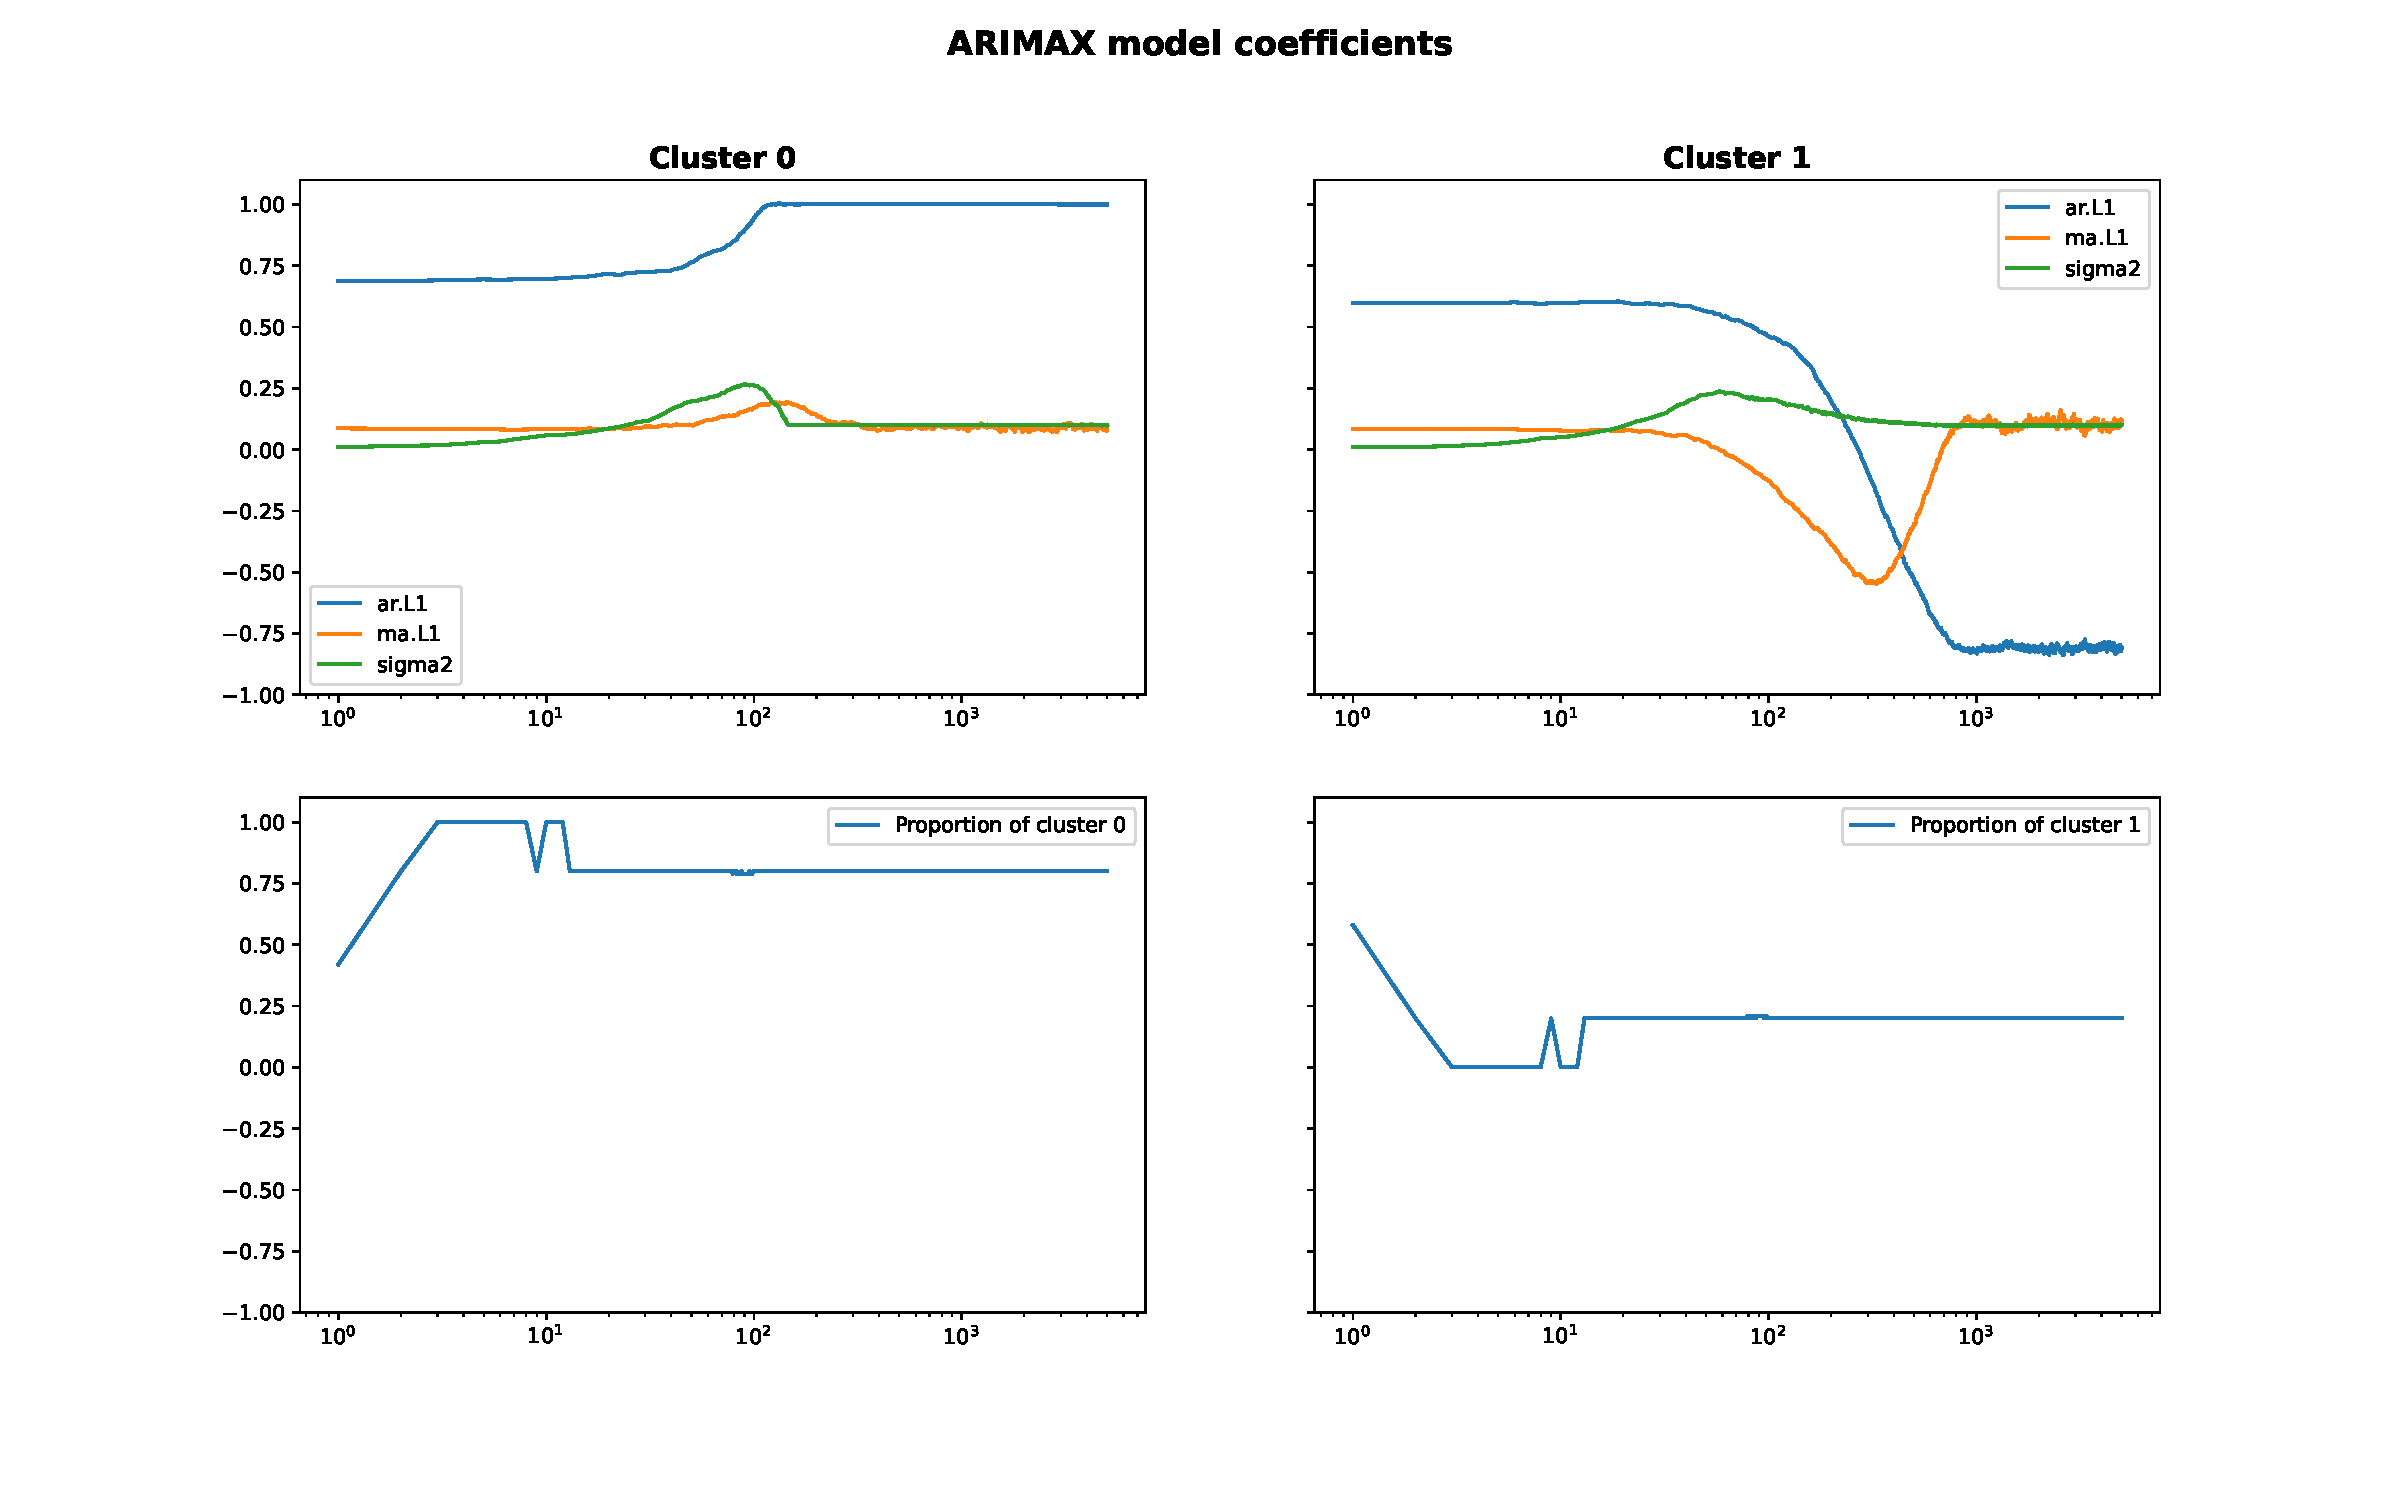
\includegraphics[width=10cm]{images/model1_graph.pdf}
    \caption{Evolution au cours des simulations de l'estimation de $\alpha$, $\beta$, $\sigma^2$, $S$ et $\phi$ pour chaque cluster pour le modèle 1}
\end{figure}
\newline 
On remarque que les paramètres convergent vers leur vraie valeur autour de la 1000ème simulation.

\subsection{Modèle 2}

Le deuxième modèle consiste en un ARMAX(1,1) de la forme : 

\begin{equation*}
y_{i,t} = \alpha_{S_i}y_{i,t-1} + \beta_{S_i}\epsilon_{t-1} + \gamma_{S_i}x_t + \epsilon_t
\end{equation*}

Ici, $\theta_k$ = $(\alpha_k,\beta_k,\gamma_k)$ où $\alpha_k$, $\beta_k$ et $\gamma_k$ sont respectivement les paramètres AR(1), MA(1) et le coefficient devant la variable exogène des séries temporelles appartenant au cluster $k$. Le processus $x_t$ est une marche aléatoire et est observé.


On fixe K = 3 et N = 100, et on utilise les mêmes priors que dans le modèle 1 : 

Puisque $\epsilon_t \sim \mathcal{N}(0,\sigma^2)$ avec $\sigma^2$ connue, on a :

\begin{equation*}
y_{i,t}|y_{i,t-1},..,y_{i,0},\theta_{S_i} \sim \mathcal{N}(\alpha_{S_i}y_{i,t-1} + \beta_{S_i}\epsilon_{t-1} + \gamma_{S_i}x_t, \sigma^2) 
\end{equation*}

Dès lors, nous sommes capables de calculer les posteriori (4), (5) et (6) et pouvons estimer les paramètres à l'aide de la méthode décrite dans la partie 2.
\newline
Voici les résultats que nous obtenons après 5 000 itérations : 
\newline
\begin{small}
\begin{center}
\begin{tabular}{|c|c|c|c|c|c|c|c|}
        \hline
        \textbf{Coefficients} & $\alpha$ & $\beta$ & $\gamma$ & $\sigma^2$ &Taille des clusters\\ 
        \hline
        Vraie valeur & 1, -0.8, 0.5  & 0.1, 0.1, 0.5 & 0.1, 0.5, 0.9 & 0.1 0.1 0.1 & 60, 20, 20 \\ 
        \hline
        Valeur estimée & 0.99 -0.75 -0.50 & 0.11, 0.03 0.55 & 0.091, 0.497, 0.886 & 0.099 0.097 0.098 &60, 20, 20\\
        \hline
        Erreur (\%) & 0.07\% 6.88\% 0.56\% & 14.29\% 70.58\% 9.35\% & 9.4\%, 0.57\%, 1.54\% & 0.46\% 2.03\% 1.32\% &0\%, 0\%, 0\%\\
        \hline
\end{tabular} 
\end{center}
\end{small}
\vspace{0.4cm}
\newline 
Notre modèle a parfaitement attribué à chaque série son cluster, et il a très bien estimé les paramètres $\alpha$ et $\gamma$ au sein de chaque cluster. En revanche, on remarque qu'il a été moins bon en ce qui concerne le paramètre $\beta$ (MA(1)). Peut-être qu'en choisissant un prior plus pertinent l'erreur aurait été moins importante.
\newline
Les graphiques ci-dessous nous permettent de visualiser la convergence des paramètres $\alpha$, $\beta$, $\gamma$ et $\phi$ au cours des itérations pour chaque cluster.

\begin{figure}[h]
    \centering
    \includegraphics[width=15cm]{images/model3_graph.pdf}
    \caption{Evolution au cours des simulations de l'estimation de $\alpha$, $\beta$, $\sigma^2$, $\gamma$, $S$ et $\phi$ pour chaque cluster pour le modèle 2}
\end{figure}

On remarque que les paramètres convergent vers leur vraie valeur autour de la 1000ème simulations.

\section{Conclusion}
En utilisant une approche bayésienne et des méthodes de Monte Carlo, nous avons réussi à grouper au sein de différents clusters des séries temporelles. Nous avons pu remarquer que les estimations des paramètres AR étaient très proche des vraies valeures et que nos algorithmes ne faisaient pas d'erreur de classification, en revanche les estimations des paramètres MA étaient souvent moins pertinentes. Cela vient de part de la difficulté d'estimation des paramètres propres aux modèles ARIMA. D'autres part, nous sommes partis de l'hypothèse que tous les paramètres suivent la même loi à priori.
\newline 
Dans un soucis de simplicité, et afin de juger la méthode uniquement sur un plan théorique, nous avons travaillé avec des données simulées. La méthode que nous avons mise en oeuvre et qui est décrite par les chercheurs semble cependant donner des résultats probants. Il serait intéressant d'étudier les performances sur des données réelles, comme des trajectoires économiques de pays ou bien des variations d'actifs financiers. 


